\documentclass[12pt]{article}
\usepackage[left=0.8in,right=0.8in,top=0.8in,bottom=1.2in]{geometry}
\geometry{a4paper}
\usepackage{graphicx}
\usepackage{amssymb}
\usepackage{fancyhdr}
\usepackage{booktabs}
\usepackage{setspace}
\usepackage{amsmath,mathrsfs}
\usepackage{multicol}
\usepackage{amssymb}
\usepackage{algpseudocode}
\usepackage{graphicx}
\usepackage{subfig}
\usepackage{subcaption}
\usepackage{array}
\usepackage{xcolor}
\usepackage{float}
\usepackage{enumitem}
\usepackage{mathcomp}
\usepackage{tabularx}
\usepackage{wasysym}
\usepackage[all,matrix]{xy}
\usepackage{multirow}
\usepackage{enumitem}
\usepackage[
    colorlinks, 
    linkcolor=blue, 
    citecolor=green]{hyperref}
\usepackage{parskip}
\usepackage[sort&compress]{natbib}
\DeclareMathOperator*{\argmax}{arg\,max}
\DeclareMathOperator*{\argmin}{arg\,min}
\usepackage{tikz}
\usepackage{mathtools}
\newcommand{\E}{\mathbb E}

\title{Duelling DQNs for Datacenter Cooling}
\author{Joseph Islam, Peyton Gozon, Aadarsha Gopala Reddy}
\date{12 December, 2024}

\begin{document}
\maketitle

\section{Introduction}

With deep learning's popularity soaring in the 2010s, and with companies increasingly turning towards big data, data centers have increasingly become part of the functioning of the modern world. As data center usage has grown, so has the associated energy consumption -- both in terms of operating the computers and cooling the environment. This growing energy consumption has highlighted the need to reduce operational costs and environmental impact. Although large-scale data centers have been studied extensively, small- to mid-sized data centers remain understudied -- despite occupying 42.5\% and 19.5\% of the market share, respectively~\cite{brightlio_data_center_stats}. 

As machines within a data center complete their tasks, they generate heat; with machines occupying physical spaces, this creates a complex spatial cooling problem within the data center. Special care also must be taken to account for the external (changing by season) weather of the data center. Given the spatial distribution of machines and data centers often having multiple cooling elements distributed throughout the space, this becomes a complex control task.

Deep Reinforcement Learning (DRL) represents a promising technique to address these issues. With its ability to dynamically adapt to changing conditions, such as machine workload and external temperature, and its ability to learn from continuous feedback, DRL offers flexibility that's lacking in static rules-based methods. Furthermore, given DRL's capacity for robust decision-making, and its ability to account for non-linear relationships among sensor readings and uncertainties about future workloads, it seems poised to outperform control-based methods.

This project leverages Deep Reinforcement Learning (DRL) to optimize the energy efficiency of cooling  small- to mid-sized data centers. We provide a comparative analysis of Proximal Policy Optimization (PPO), Soft Actor-Critic (SAC), and Dueling Deep Q-Networks (DDQN) in this domain, and compare their efficacy against static rules-based and control-theoretic baselines. 

Key contributions include: 
\begin{itemize}
    \item A focus on small- to mid-sized data centers
    \item A novel exploration on DDQN within for data-center cooling
    \item Comparisons between DRL methods with a rules-based and control-theoretic controller
\end{itemize}

% The growing energy consumption of data centers has highlighted the need for efficient cooling systems to reduce operational costs and environmental impact. While large-scale data centers have been extensively studied, small to mid-sized data centers remain underrepresented in research despite occupying a sizable market share~\cite{brightlio_data_center_stats}. This project leverages Deep Reinforcement Learning (DRL) algorithms—Proximal Policy Optimization (PPO), Soft Actor Critic (SAC), and Dueling Deep Q-Network (DDQN)—to optimize cooling in small to mid-sized data centers using EnergyPlus simulations to show the promise of the unresearched DDQN for data center cooling.

% The main contributions of this work include a comparative analysis of PPO, SAC, and DDQN in the context of random and rules based cooling optimization baselines, a novel focus on small to mid-sized data centers, an underexplored market segment, and insights into the practicality and convergence of DRL algorithms using EnergyPlus simulations. Key challenges include limited granularity in control systems, data availability for model training, and computational constraints in small facilities.

\section{Related Works}

% Write your literature review here. Summarize existing work, research, or methodologies related to your project. Highlight gaps your project aims to address and the main difference between your project and previous work.

The data center cooling research and practice currently seem immature. Small data centers occupy approximately \textbf{42\%} of the data center market~\cite{brightlio_data_center_stats}, which is expected to grow by \textbf{12.5\%} in the next eight years~\cite{gminsights_data_center_growth}. While Google DeepMind~\cite{deepmind_cooling} and DeepEE~\cite{deepee} have explored cooling optimization for large data centers, Dominkovic et al.~\cite{cool_data_project} acknowledge that addressing market growth's threat to decarbonization goals needs more research in small-to-mid-sized data center cooling optimization. Contrastive studies featuring DQN, BDQ, and DDPG~\cite{song2021comparison}, model-based reinforcement learning, and PPO~\cite{zhang2019building}, SAC~\cite{sac_comparitive_paper}, as well as separate frameworks like Cool.Ai~\cite{cool_ai_framework} have been researched, but overlook common methods like Duelling Deep Q Networks, which we explore. We leverage the EnergyPlus simulation environment~\cite{energyplus} via the Sinergym Python wrapper~\cite{sinergym_github}, as demonstrated in prior work~\cite{sinergym_paper}, to evaluate the applicability of SAC, DDQN~\cite{wang2016dueling}, and PPO for small to mid-size data center cooling systems to review alternative DRL algorithm's applicability to data center cooling.


\section{Background \& Preliminaries}

Data centers are large facilities housing computing devices that generate heat as they process workloads. Maintaining suitable cooling conditions is critical, both in terms of operational efficiency and hardware longevity, but also for occupant safety. Finding an energy-efficient cooling strategy, however, is a complex challenge due to the non-linear and time-dependent interactions between server workloads, environmental conditions, cooling elements, and the spatial relationship between them.  

Reinforcement Learning (RL) provides a promising framework for addressing this challenge. In RL, an agent interacts with an environment, which is modeled as a Markov Decision Process (MDP). An MDP is defined as a 4-tuple, $(\mathcal S, \mathcal A, \mathcal T, \mathcal R)$, where $\mathcal S$ is the set of states, $\mathcal A$ is the set of actions, $\mathcal T : \mathcal S \times \mathcal A \to \mathcal S$ defines the transition function mapping $(s, a) \mapsto s'$, and $R$ defines the reward function. At time step $t$, the agent observes state $s_t \in \mathcal S$, and selects action $a_t \in \mathcal A$ according to the transition function, and receives reward $r_t$ reflecting how good the resulting state is. We seek to find a policy, that is an optimal set of actions for each state, such that we maximize the cumulative rewards over time. Future state rewards are discounted by $\gamma$. 

In the data center cooling problem, states correspond to the readings of sensors placed both in and around the facility -- such as internal or external thermometers, humidity sensors, and wind direction and speed information. Additional information might also be added to this vector, such as (remaining) workloads of machines. 

Actions, in this setting, correspond to interactions with cooling elements throughout the facility -- such as turning on or off HVAC systems, or setting fan speeds. Ideally, the action taken $a_t$ utilizes the cooling elements efficiently.

The problem then, at its core, is to uncover the model of the data center cooling problem, $T(s, a)$. This can be highly complex, especially as the spatial layout of the sensors, computers, and cooling elements are considered -- not to mention the non-linear relationship with humidity, outdoor temperature, and the time-delay between activating an HVAC system and observing the temperature be corrected. Recovering $T$ is thus the crux of the problem. 

Many algorithms exist to facilitate this -- in this paper, we will investigate Proximal Policy Optimization (PPO), Soft Actor-Critic (SAC), and Dueling Deep Q-Networks (DDQN) to implicitly learn this model. Before we can investigate these methods, we must also consider how to evaluate the current state of the environment. This is defined as $R_t$, or the ''Reward" at the current time step $t$. For the purposes of this exploration, we consider a reward function, $R(s_t)$, that balances between energy consumption and the difference between the current temperature and a ``comfortable" temperature. The specifics of how these are balanced will be addressed in the Methods section. 

We specifically choose to explore the novel application of DDQN to datacenter cooling in the context of already applied DRL algorithms PPO and SAC to provide an elementary contrastive study accessible to industry practitioners trying to optimize their data center cooling.

% The control problem is formulated as a Markov Decision Process (MDP) to optimize data center cooling. State space is a vector over floats describing environmental properties like temperature, humidity, extended by weather forecasting information from EnergyPlus. The continuous action space consists of floats from min and max intervals that specify a range to keep HVAC temperature within for that time period. The Reward Function is a ratio that balances energy efficiency and thermal comfort per the formula $R(s,a)=R_{energy}+R_{comfort}$. The transition function defines the probability of transitioning to a new climate state s', given the current climate state s, when an HVAC action is taken. The discount Factor $\gamma$ balances present and future focus for the model's decision making and learning. The objective is to find a policy that maximizes the expected cumulative discounted reward across the episodes.

% High dimensionality in the real-time climate, input, or state space combined with data center workload uncertainty and incomplete sensor information challenge fitting a theoretical MDP to the real world for even small data centers beyond the complications of just tthermal inertia. Intentional model selection allows us to overcome this. A successful DRL solution will optimize beyond the improvements that standard, human-implemented symbolic rule-based incremental and rule-based controllers like Sinergym's see over random baselines. Such controllers often respectively define acceptable static condition intervals to control for, e.g. temperature between 18 and 30 degrees celsius, or define acceptable condition ranges around a moving, environmentally driven target, as in the incremental context to maintain temperature within 10 degrees celsius of the temperature outside. Performance beyond the limits of these deterministic solutions' indicates success for DRL systems, lest they fail to outperform human effort. For success, we chose PPO, SAC, and DDQN.

% We choose PPO and SAC because they are state of the art in DRL for continuous action spaces in stochastic environments. We choose these alongside the well understood and widely used, but not yet applied to data center cooling, DDQN, offering a novel contribution. While DDQN is not a natural fit for data center cooling, minor adaption to discretizing the continuous control space to enable DDQN to work promises DDQN's reliability despite the complexities imposed by thermal inertia. Placing DDQN in the context of field-familiar PPO and SAC for data center cooling empowers data center owner decision making with modern, well-contextualized contrastive study results. Performance of our models beyond the rule based methods suggests owners to use DRL to optimize their cooling, rather than simpler existing rule-based techniques. 

\section{Method}

We first discuss the simulator setup (Section~\ref{method:sim}), then our RL problem formulation (Section~\ref{method:drl_setup}), followed by implementation details for each algorithm (Section~\ref{method:algo_details}), baselines (Section~\ref{method:baseline}), real-world training and computer-environment details (Section~\ref{method:practical}).

\subsection{Simulator}\label{method:sim}
We use the \texttt{Sinergym} Python package to simulate the dynamics of a small datacenter. \texttt{Sinergym} is a Gymnasium-compatible wrapper for \texttt{EnergyPlus}, which is "a whole building energy simulation program that engineers, architects, and researchers used to model ... energy consumption ... in buildings"~\cite{energyplus}. Having this tool accessible through a Gymnasium-compatible wrapper allowed our group to adapt to this complex domain with a familiar programming context. 

We chose to use \texttt{Sinergym}'s built in \texttt{Eplus-datacenter-mixed-continuous-stochastic-v1} environment. According to Sinergym's documentation~\cite{sinergym_github}, this environment simulates a "491.3 $m^2$ building, divided into two asymmetrical zones: the west zone and the east zone. Each zone is equipped with an HVAC system. The primary heat source in the building is generated by the hosted servers". 

\begin{figure}[h!]
    \centering
    \includegraphics[width=0.5\linewidth]{images/datacenter.png}
    \caption{Sinergym 2-Zone Datacenter with HVAC}
    \label{fig:datacenter}
\end{figure}

This environment, being "mixed," will choose between hot and cold temperature data to be simulated on a given run. This environment is also stochastic, meaning that weather fluctuations are amplified by an additional 1.5 standard deviations of normal conditions. This was chosen to ensure our DRL algorithms work across a robust set of conditions. 

By default, \texttt{Sinergym} utilizes a linear reward function. This is defined as, 

\[R(t) = -W \cdot \lambda_E \cdot \mathrm{Power}_t + (1 - W) \cdot \lambda_T * (\max(T_t - T_\mathrm{low}, 0) + \max(T_\mathrm{upper} - T_t), 0)\]

where, $\lambda_E = 1$ is an energy-specific weighting term, $\lambda_T = 1$ is an energy-specific weighting term, and $W \in [0, 1]$ considers the balance. $T_\mathrm{lower}$ and $T_\mathrm{upper}$ are the lower- and upper-temperature bounds considered comfortable, with $T_t$ being the current temperature. 

As a simplifying assumption, we only train our algorithms across the period of June 1st to August 31st in a given year. This was chosen as it represents the period with the greatest volatility in terms of temperature, making rewards less sparse. 

By default, the weather file used by \texttt{EnergyPlus} used weather details sampled from JFK International Airport. 

\subsection{Reinforcement Learning Setup}\label{method:drl_setup}

By default, the state space of this environment is 28-vector of different environment properties, including the internal temperature of both the west and east zones, as well as their humidities, and the outdoors conditions. See Appendix~\ref{App:ss} for a complete overview of state-space variables. 

During the ablation study, we also wrap the environment in \texttt{Sinergym}'s \texttt{WeatherForecastingWrapper}. This provides weather information three days into the future, with each day being represented as another six floats appended onto the original state space; thus, when the wrapper is enabled, our state space becomes a 46-vector. 

The action space is a 2-vector, codified as the $\begin{bmatrix}
    \text{lower-threshold} & \text{upper-threshold}
\end{bmatrix} \in [15, 22] \times [22, 30]$ sets the temperature control boundaries. If the indoor temperature (in a given zone) falls below the lower-threshold, heating initiates; if it rises above the upper-threshold, cooling is activated. Each of these values are temperatures in Celsius. When an action is applied to the environment, both the HVACs controllers are given the action's temperature control boundaries. 

\subsection{Algorithmic Details} \label{method:algo_details}

We implemented PPO, SAC, and DDQN DRL algorithms for this problem. However, we made alterations to each algorithm to make it work within the environment. 

\subsubsection{PPO Implementation Notes}
PPO is implemented with two implicit neural networks, a Policy Network and a Value Network. Both networks are feed-forward sequential networks with ReLU non-linearity, with the Policy Network returning a mean and standard deviation (defining a policy distribution) for a given state; the Value Network estimates the value of the state. Both are optimized using Adam.

Internally, each element of the action vector is scaled to $[-1, 1]$ to improve stability by $\tanh$-squashing. Actions are rescaled to the bounds identified above whenever they are used to interact with the environment. 

After consulting the literature, we identified Generalized Advantage Estimation (GAE) as a way to improve training stability. This method uses the TD($\lambda)$ algorithm to calculate a $\lambda$-return to compute the Generalized Advantage Estimator, $\mathrm{GAE}(\lambda)$~\cite{schulman2015high}: 
\[\hat{\mathcal{A}_t} = \mathrm{TD}(\lambda) - V(s_t)\]

We found the details in Appendix (A) of~\cite{peng2018deepmimic} particularly insightful. 

Exact learning rate, clip ratios, mini-batch sizes, and neural network architectures are modified in each experiment. 

\subsubsection{SAC Implementation Details}

Our implementation of SAC utilizes a single actor with two critic networks to improve stability with training. Just like in PPO, the policy network computes the mean and standard deviation of the policy distribution for a given state through a feed-forward network with two heads. The critic networks are also feed-forward networks Q-networks with ReLU activation functions. All three networks are optimized using Adam. 

SAC, similar to our PPO implementation, uses $\tanh$-squashing to improve training stability internally; all interactions with the environment are scaled to the environment's action space. 

We also implemented automatic entropy tuning to balance exploration vs exploitation, making SAC perform more effectively in our environment. (In fact, we found SAC performed poorly without it). We optimized this parameter using Adam as well. 

We use soft-updates with $\tau = 0.005$ for each minibatch update. 

\subsubsection{DDQN Implementation Details}

This is perhaps the most interesting. DDQNs, given a state, choose between a series of discrete actions; however, our environment is continuous. 

To overcome this, we discretize the action space, converting the domain of the lower-threshold and upper-threshold into a series of five bins of equal width; this means $|\mathcal A| = 5 \times 5 = 25$ for the DDQN. 

The DDQN is defined very similarly to its original paper~\cite{wang2016dueling}. However the original paper is designed to operate on the Atari Gym environment. To this end, we took liberty with designing the feature stream as a feed-forward neural network with one hidden layer, rather than the series of 2D-convolutional layers depicted in the original paper. Faithful to the original implementation, we then use the feature-stream to compute two separate streams -- a value stream and an advantage stream -- before combining the values together again to compute the Q-values for each action. 

We used a linearly decaying epsilon GLIE policy to handle the exploration vs exploitation trade off. 

\subsection{Baseline Details}\label{method:baseline}

We explored three baselines, each available through \texttt{Sinergym} by default. 

As is a common baseline, we evaluated the \texttt{RandomController}, which samples a random action from the environment's action space at each time step. 

For a static rule-based baseline, we utilized the \texttt{RBCDatacenter} controller (Rules-based Controller for the Datacenter environment). This always selects an action of $(18, 27)$ celsius, corresponding to The American Society of Heating, Refrigerating and Air-Conditioning Engineers (ASHRAE) guidelines. 

For a control-theoretic approach, we used the \texttt{RBCIncrementalDatacenter} controller. This begins by using the \texttt{RBCDatacenter} Controller's action of $(18, 27)$, but varies the upper- and lower-thresholds according to the average temperature of the west- and east-zones in the data center. If the mean indoor temperature exceeds the `upper-threshold`, both the lower- and upper-thresholds are decreased by one degree centigrade; conversely, if the lower-threshold exceeds the mean indoor temperature, both the lower- and upper-thresholds are increased by one. This controller stabilizes internal temperature in an energy-efficient way through a series of one-degree increments to the temperature set points 

\subsection{Experimental Infrastructure}\label{method:practical}

We implemented all our models using PyTorch, performed model convergence analysis using Tensorboard. Our environment specifics are a fresh Conda 3.1.2 environment running Python 3.12, torch 2.5.1, tensorboard 2.18.0, wandb 0.19.0, gymnasium 1.0.0, sinergym 3.7.0 (installed directly via GitHub~\cite{sinergym_github}, and EnergyPlus 24.2.0.

We ran our models across 14 M2 Mac Minis, usually overnight. We analyzed the average per-step reward for evaluation, but looked at the total episode reward to understand model performance while training; as one full episode is consistently defined as $6624$ steps, we could convert between these values as necessary. 

\begin{figure}[h!]
    \centering
    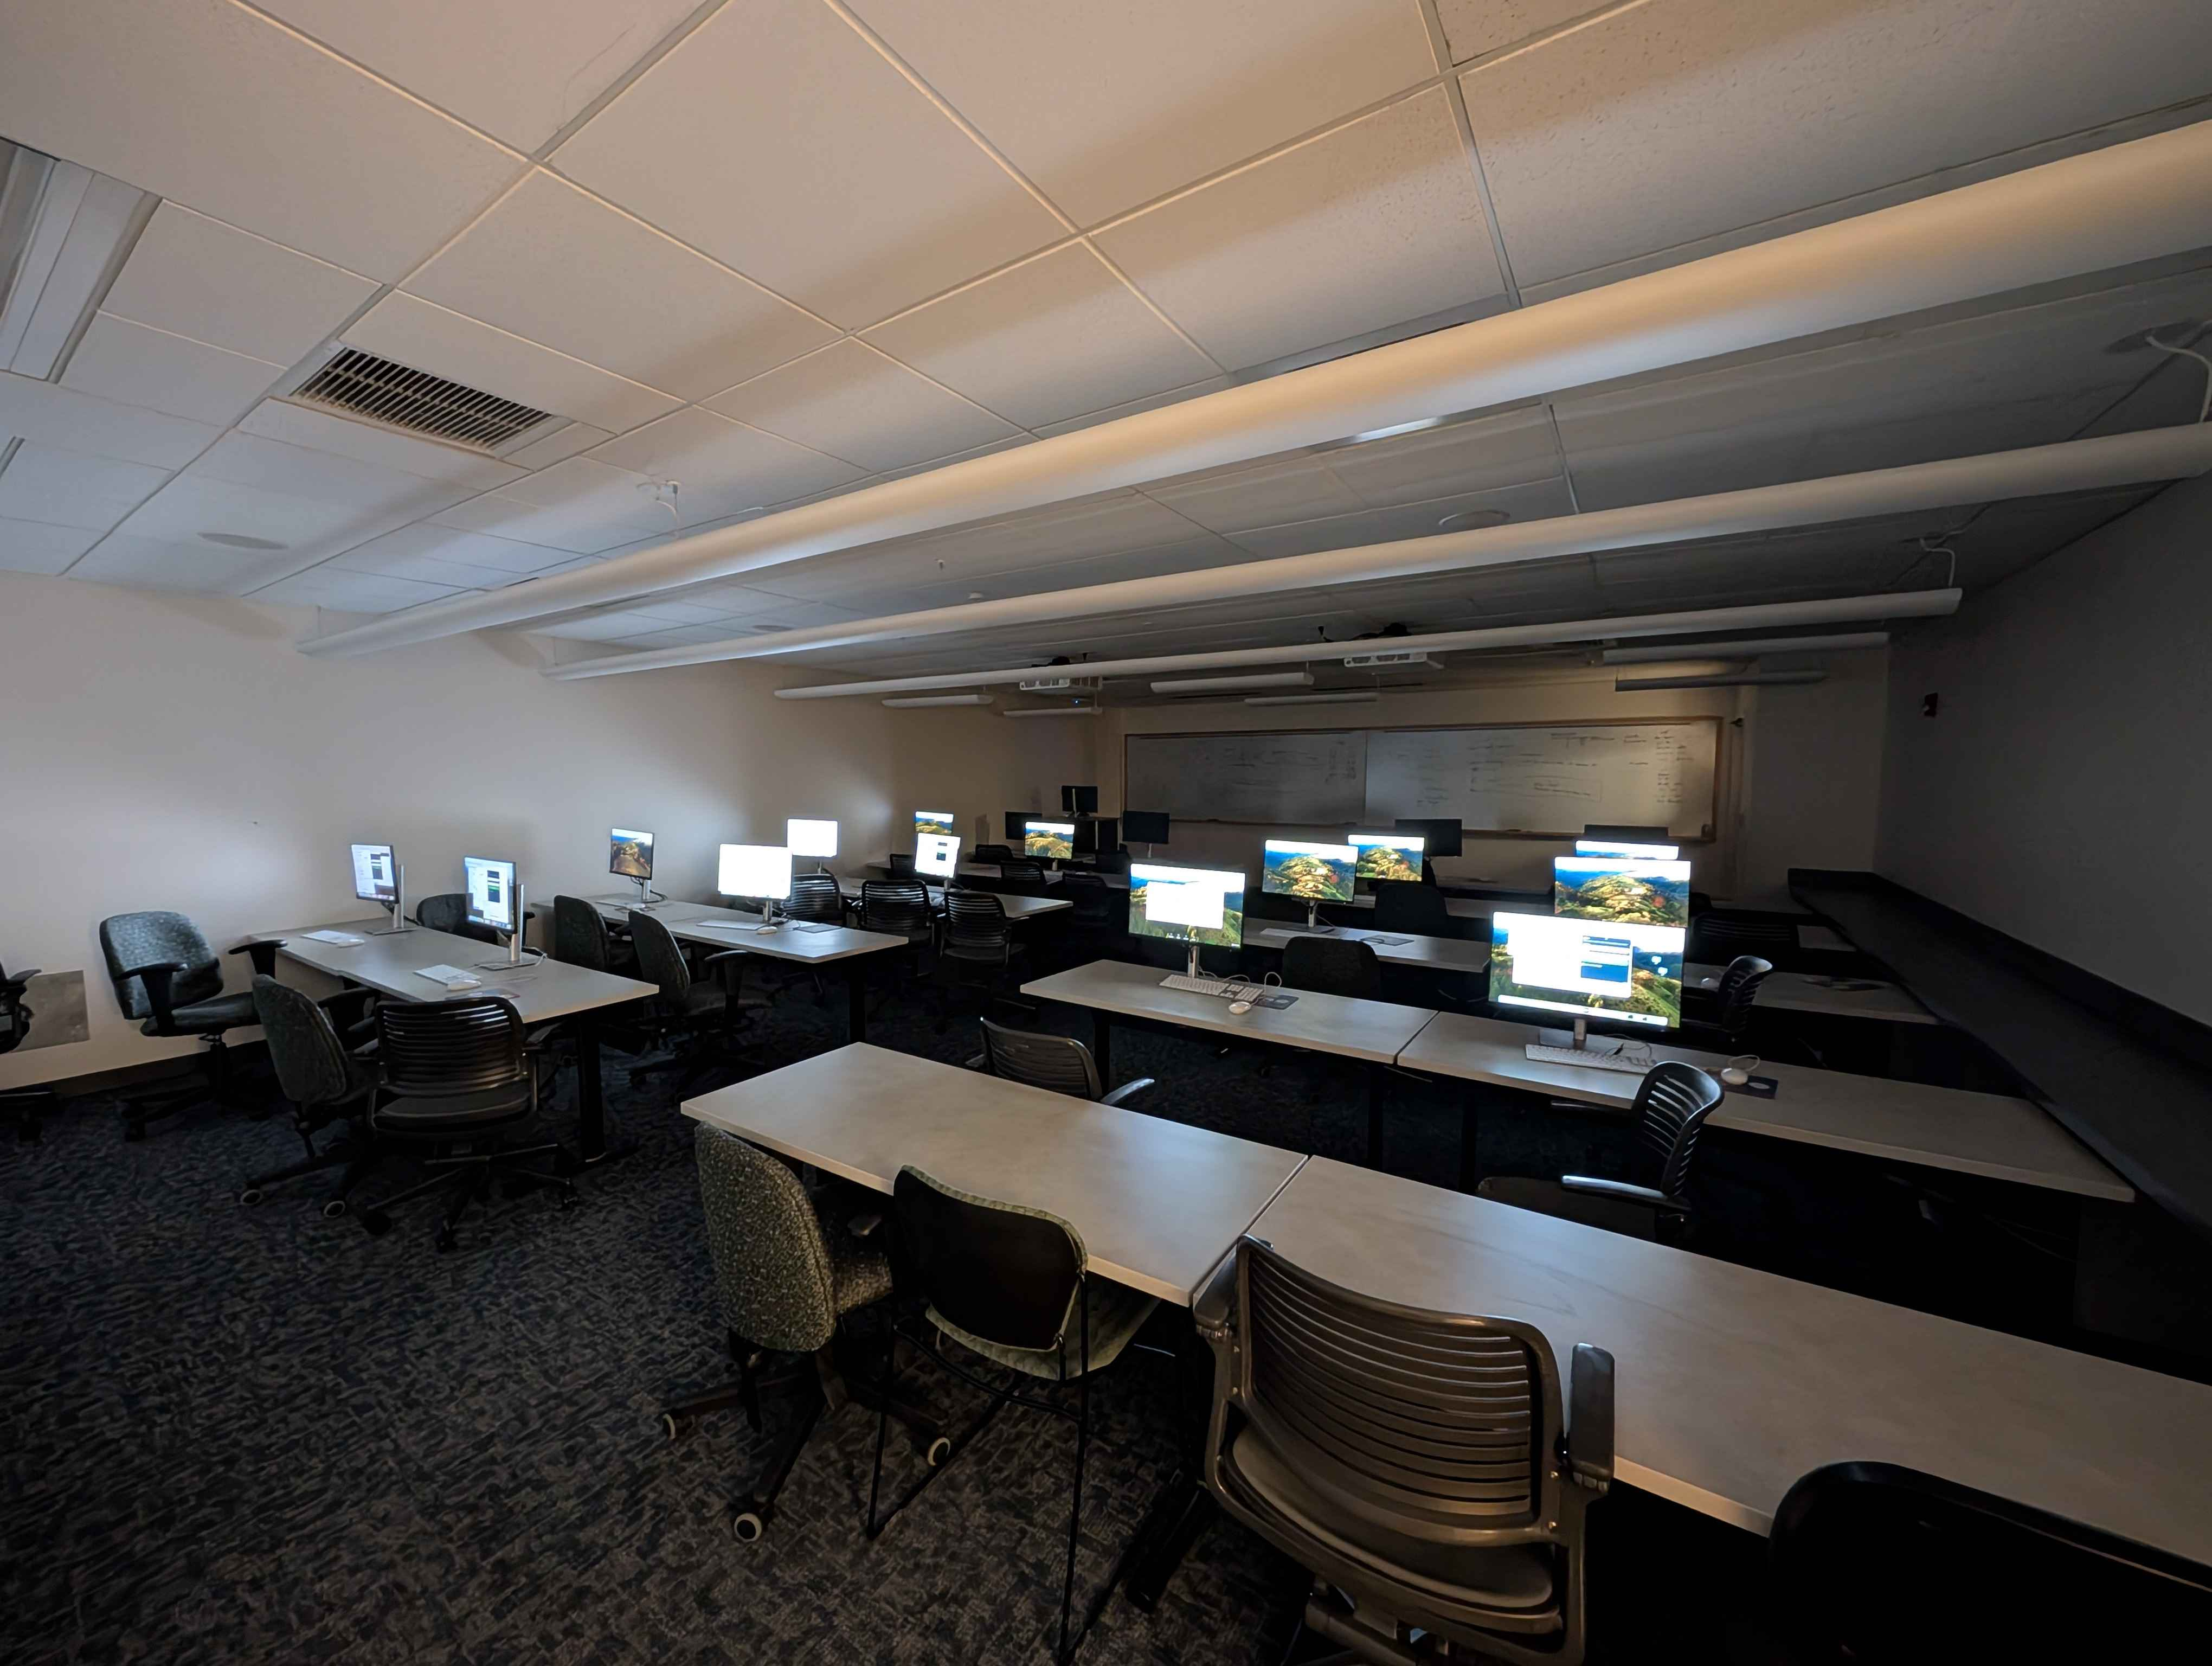
\includegraphics[width=0.5\linewidth]{images/PXL_20241211_072647623.png}
    \caption{Training Overnight. Ironic how we made a data center, while learning how to cool them.}
    \label{fig:training_overnight}
\end{figure}


\section{Experiments}

We conceptualized the experiments as three separate investigations into data center cooling, one for PPO, SAC, and the DDQN. Our primary goal in running these experiments was to explore whether they would outperform the Random Baseline, the static Rules-Based Baseline, and the control-theoretic Rules-Based Incremental Baseline. 

All experiments were conducted in the simulated data center environment, across the time period of June 1 to August 31. 

We began by performing a partial grid search with refinements to identify key model parameters that would lead to model convergence. Once these models were identified, we performed hyperparameter tuning on the models. We evaluated models in terms of their average per-timestep reward during an evaluation setting. Model performance was averaged across 20 evaluation episodes.  Models were evaluated every 10 episodes while training. 

These are the parameters domains evaluated for each model:
\subsubsection{PPO}
\begin{itemize}
    \item learning rate $\in [10^{-4}, 3\cdot10^{-4}, 10^{-5}]$
    \item learning rate scheduler $\in [\text{Linear}, \text{Exponential}]$
    \item number of hidden layers $\in [2, 3, 4]$
    \item nodes per hidden layer $\in [64, 128, 256]$
    \item batch size $\in [64, 128]$
    \item clip ratio $\in [0.1, 0.2, 0.3]$
    \item Include 3-day Weather Forecasting? $\in [\text{Yes}, \text{No}]$
\end{itemize}

We also specified $\lambda = 0.95$ for computing GAE. PPO was evaluated for $50$ epochs, at $6624$ steps per episode. 

\subsubsection{SAC}
We chose to limit our exploration of SAC to neural networks with two hidden layers, kept the soft-update parameter $\tau = 0.005$ fixed. We also instantiated the Replay Memory to have a buffer capacity of $1,000,000$. 
\begin{itemize}
    \item learning rate $\in [10^{-3}, 3 \cdot 10^{-3}]$
    \item learn entropy? $\in [\text{Yes}, \text{No}]$
    \item $\gamma \in [0.99, 0.995]$
    \item nodes per hidden layer $\in [128, 256]$
    \item number of initial episodes to sample for replay memory $\in [3, 5]$
    \item target model update frequency $\in [25, 50]$
    \item batch size $\in [64, 256]$
\end{itemize}

SAC was evaluated for 100 epochs. 

\subsubsection{DDQN}
For the DDQN, we chose to vary the following parameters:
\begin{itemize}
    \item learning rate $\in [10^{-3}, 5 \cdot 10^{-4}, 2.5 \cdot 10^{-4}, 10^{-5}]$
    \item steps until max learning rate decay $\in [50000, 100000, 200000]$
\end{itemize}

We fixed the initial epsilon, used for the GLIE policy, to be $1.0$ with us linearly decaying to $0.1$ over the steps specified above. We fixed $\gamma = 0.99$, the network architecture to have $64$-nodes per hidden layer. The replay memory, like in SAC, had a maximum capacity of $1,000,000$. We performed a hard model update every $10$ episodes. The DDQN was evaluated for a maximum 300 episodes, or until it achieved a performance of $-12300$; note, this level of performance beat all the baselines. 

\subsubsection{Ablation Study}

Finally, we chose to perform an ablation study on our novel contribution, using DDQN for data center cooling. In this study, we chose four well-performing models from the DDQN subsection, and decided to see whether including a three-day weather forecast improved model performance. We chose to study the inclusion of the weather forecasting information on the DDQN in particular, partially as a continuation of the work done for PPO, but also because the DDQN models are drastically simpler than PPO or SAC, outperformed PPO and SAC, and deserve more coverage since they're our novel contribution.

% ===== IYO SEPARATOR =====


% Describe your experiments setting here, including compared methods, the evaluation metrics, data source, data amount, hyper-parameters, etc. Show your results and have some analysis about the results.
% It is better for this section to include some additional experiments to demonstrate aspects such as the effectiveness of each part of the method (ablation study) and the motivation behind the method (didactic example), among others.

% Our initial experiments primarily focused on comprehensively exploring hyperparameters involved in PPO, SAC, and DDQN. For PPO, we explored all configurations of 2, 3, and 4 hidden layers with 64, 128, and 256 nodes against clip ratios of .1, .2, and .3, batch sizes of 64 and 128, and linear or exponential learning rate scheduling from a base learning rate of either .0003 or .00001. For SAC, we explored gamma of .99 and .95, a fixed and exponentially decaying learning rate of .2 or decaying at .99, eta at .0003, 5 or 3 for RB updates, 25 or 50 steps for update frequency, and batch size of 4 on a baseline network of 2 layers with 256 nodes each. We also explored these SAC configurations against another architecture of 2 layers with 128 nodes each, a batch size of 256, and a learning rate decay of .995. We explored a learning rate of .001, .00025, .0001 and learning rate decay over 50 and 200 thousand time steps for our discretized DDQN. Totaling over 100 experiments, this parameter search domain was intentionally selected to promote model performance and accelerate convergence, evaluated by number of episodes required to show limited improvement in the recent running reward average against the current episode's reward, both in daily and cumulative contexts.


\subsection{Results and Analysis}

\begin{figure}[h!]
    \centering
    \includegraphics[height=0.5\textheight, width=1\textwidth, keepaspectratio]{images/graph__.png} % Replace with your image path
    \caption{Models against baselines on small mixed continuous stochastic energyplus data center. }
    \label{fig:maincomparison}
\end{figure}

\begin{table}[ht]
\centering
\caption{Final Performance by Model}
\label{tab:datatable}
\begin{tabular}{|l|c|c|c|}
\hline
\textbf{Model Name} & \textbf{Total Reward} & \textbf{Average Reward} & \textbf{\%} \\ \hline
DDQN                & -12130                     & -1.835                       & 35.8           \\ \hline
PPO               & -12496                     & -1.893                       & 10.9           \\ \hline
SAC                & -12630                     & -1.916                       & .284           \\ \hline
RBC-INC                & -12634                     & -1.907                       & 0           \\ \hline
RBC            & -13753                     & -2.08                       & -           \\ \hline
Random             & -14042                     & -2.2                       & -           \\ \hline
\end{tabular}
\end{table}


Figure~\ref{fig:maincomparison} shows the training curves of our models, contextualized by the performance of the baseline models averaged across the episodes. Table~\ref{tab:datatable} shows the cumulative final rewards across episodes and averaged by days for these models. The percentage column describes the percentage improvement our model had beyond the improvement that RBC-INC made over the random baseline. We expected our PPO and SAC to perform comparably and exceed our baselines. SAC surpassed RBC-INC by .284\%, but PPO exceeded RBC-INC's improvement by 10.9\%, contradicting our comparability hypothesis. This may be due to insufficient grid searching for SAC. Most notably and surprisingly, our DDQN adaptation far surpassed PPO, at a 35.8\% improvement over RBC-INC's. We suspect this could be because of DDQN's relative simplicity compared to PPO's, but this suggests that model free DRL methods offer significant potential improvement over traditional rules based approaches for real datacenters.
Furthermore, small to mid sized datacenters struggling with high setup costs may find DDQN to be cheaper and better than PPO and SAC at the cost of slightly lost granularity, but the returns offset this concern for simpler environments, like our simulator. With richer information found in real world settings such as server thermal data, PPO and SAC offer promise for real world applications in their ability to handle more complex state spaces than our relatively simple DDQN, and given the cost constraints smaller data centers face, especially PPO. Most importantly, the novel application of DDQN to datacenter cooling demonstrates great promise.

Actionable hyperparameter takeaways include clip ratios at most .1, 64x64 node network, linear learning rate scheduling, and a batch size of 64 for optimal PPO results in our method. We found that a learning rate of .0005 decayed over 50k timesteps with a gamma of .99 yielded optimal DDQN performance, and a gamma of .99, tau of .005, alpha of .2, learning rate of .0003, (256, 2) network architecture, learnable alpha, and automatic entropy tuning yielded the best SAC for our approach.

\subsection{Ablation Study: Impact of Weather Forecasting}

To assess the impact of weather forecasting on model performance, we conducted an ablation study where we trained the DRL agents with and without access to weather forecasts to assess the necessity of weather data for performance gain.

\begin{figure}[h!]
    \centering
    \includegraphics[height=0.75\textheight, width=0.75\textwidth, keepaspectratio]{images/comparison_2x2_a_b.png} % Replace with your image path
    \caption{Models without weather data usually outperform those with}
    \label{fig:label}
\end{figure}


\textbf{Analysis:}

In our ablation study, group A and B, the red and blue lines, respectively feature DDQNs with and without 3 day weather forecast data. Group 1, 2, 3, and 4 use learning rates of .001, .00025, .00025, and .0001 with 50000, 200000, 50000, and 50000 step learning rate decays, respectively. Our results suggest that while incorporating 3 day weather forecasting usually introduces instability and restricts model performance and convergence, more work to tell the merits of weather forecasting data seems due. This doesn't necessarily imply that such forecasts are ineffective in real-world scenarios either. While weather forecast data may complicate cooling optimization in our specific DRL frameworks, it could still prove valuable for other related tasks, such as cost and workload forecasting.




\section{Conclusions}

This paper sought to contextualize a new application of Dueling DQN's for data center cooling by offering a basic contrastive study between the a standard DDQN, for this, a GAE modification PPO implementation, and SAC with automatic entropy tuning. While the latter two algorithms are common and work well, DDQN's performance, slightly faster convergence time, and relative simplicity make it an excellent contender for real life data center cooling applications. DDQN's far exceed standard performance for little expert tuning and involvement, making them an excellent choice for data center cooling optimization amidst the high and increasing data center demand. If not DDQN's, PPO with GAE modifications remain a strong choice, but SAC may be more poorly fit for real world application due to steep training and tuning requirements a growing data center may not be able to fund. Weather forecasting data unlikely helps performance, but more research is needed for conclusive results.


\section{Limitations \& Future Works}

Our project focused on model-free methods in datacenter cooling optimization. Aforementioned complementary model based methods show promise beyond model free methods and deserve further exploration. Our PPO implementation remained true to theory, but further tailoring to the problem could offer comparable performance to the DDQN. Finally, adding gradient flow based entropy management techniques to our SAC algorithm could improve and hasten convergence in SAC. Future work in these directions would sizably support data center owners and achievement of decarbonization targets down the line.

%\clearpage
\bibliographystyle{plain}  % You can use other styles like abbrv, alpha, etc.
\bibliography{citations}  % Ensure this matches the name of your .bib file

\section{Appendix}

\subsection{State Space}\label{App:ss}

\begin{multicols}{2}
\begin{itemize}
    \item Site Outdoor Air Drybulb Temperature
    \item Site Outdoor Air Relative Humidity
    \item Site Wind Speed
    \item Site Wind Direction
    \item Site Diffuse Solar Radiation Rate per Area
    \item Site Direct Solar Radiation Rate per Area
    \item Zone Thermostat Heating Setpoint Temperature
    \item Zone Thermostat Cooling Setpoint Temperature
    \item Zone Air Temperature
    \item Zone Air Relative Humidity
    \item Zone Thermal Comfort Mean Radiant Temperature
    \item Zone Thermal Comfort Clothing Value
    \item Zone Thermal Comfort Fanger Model PPD
    \item Zone People Occupant Count
    \item People Air Temperature
    \item Facility Total HVAC Electricity Demand Rate
\end{itemize}
\end{multicols}

\end{document}